59. \begin{figure}[ht!]
\center{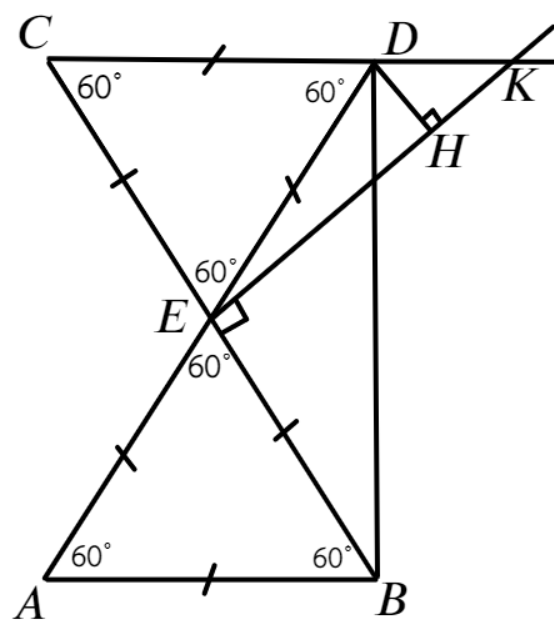
\includegraphics[scale=0.35]{g59.png}}
\end{figure}\\
Так как отрезки $AD$ и $BC$ равны и пересекаются в середине, $AE=BE=CE=DE.$ Так как $AB=CE=AE=BE,$ треугольник $AEB$ является равносторонним, а значит $\angle AEB=60^\circ=\angle DEC,$ значит треугольник $DEC$ также является равносторонним. Равные углы $DCE$ и $EBA$ являются накрест лежащими, значит прямые $DC$ и $AB$ параллельны, поэтому $\angle CDB+\angle ABD=180^\circ$ (они односторонние). $\left.\begin{array}{l}DC=AB,\\
CB=AD,\\
\angle DCB=\angle DAB  \end{array}\right\}\Rightarrow \Delta BCD=\Delta ADB\text{ по I признаку}\Rightarrow \angle CDB=\angle ABD.$ Так как $\angle CDB+\angle ABD=180^\circ,$ получаем $\angle CDB=\angle ABD=90^\circ.$ Пусть $DH$ --- перпендикуляр, опущенный из точки $D$ на $KE$ (его длина и является искомым расстоянием). Найдём $\angle DEH=90^\circ-60^\circ=30^\circ,\ \angle EDB=90^\circ-60^\circ=30^\circ,$ тогда из треугольника $DKE:\ \angle DKE=180^\circ-90^\circ-30^\circ-30^\circ=30^\circ.$ Поэтому он является равнобедренным и $DK=DE.$ В прямоугольном треугольнике $DKH$ катет $DH$ лежит напротив угла в $30^\circ,$ значит $DK=2DH.$ Таким образом, $KC=CD+DK=ED+DK=2DK=4DH,$ ч.т.д.\\
